\documentclass[12pt]{article}

\setlength{\topmargin}{-.75in} \addtolength{\textheight}{2.00in}
\setlength{\oddsidemargin}{.00in} \addtolength{\textwidth}{.75in}

\usepackage{amsmath,color,graphicx,array,multirow,rotating, enumerate}
\usepackage{type1cm}
\usepackage{eso-pic}
\usepackage[hmargin=2cm,vmargin=1.3cm]{geometry}
\usepackage{mathabx}
\usepackage[rflt]{/Users/jgates/desktop/latex/floatflt}
\usepackage[table]{xcolor}
\nofiles

\def\Tab#1{\tabular[t]{>{\rule[-1ex]{0pt}{3ex}}c}#1\endtabular}
\newcolumntype{C}{@{}c@{}}

\pagestyle{empty}
\newcounter{ProbNum}
\setlength{\parindent}{0in}

% Watermark: graph paper
\newcommand\BackgroundPic{
\put(0,0){
\parbox[b][\paperheight]{\paperwidth}{%
\vfill
\centering
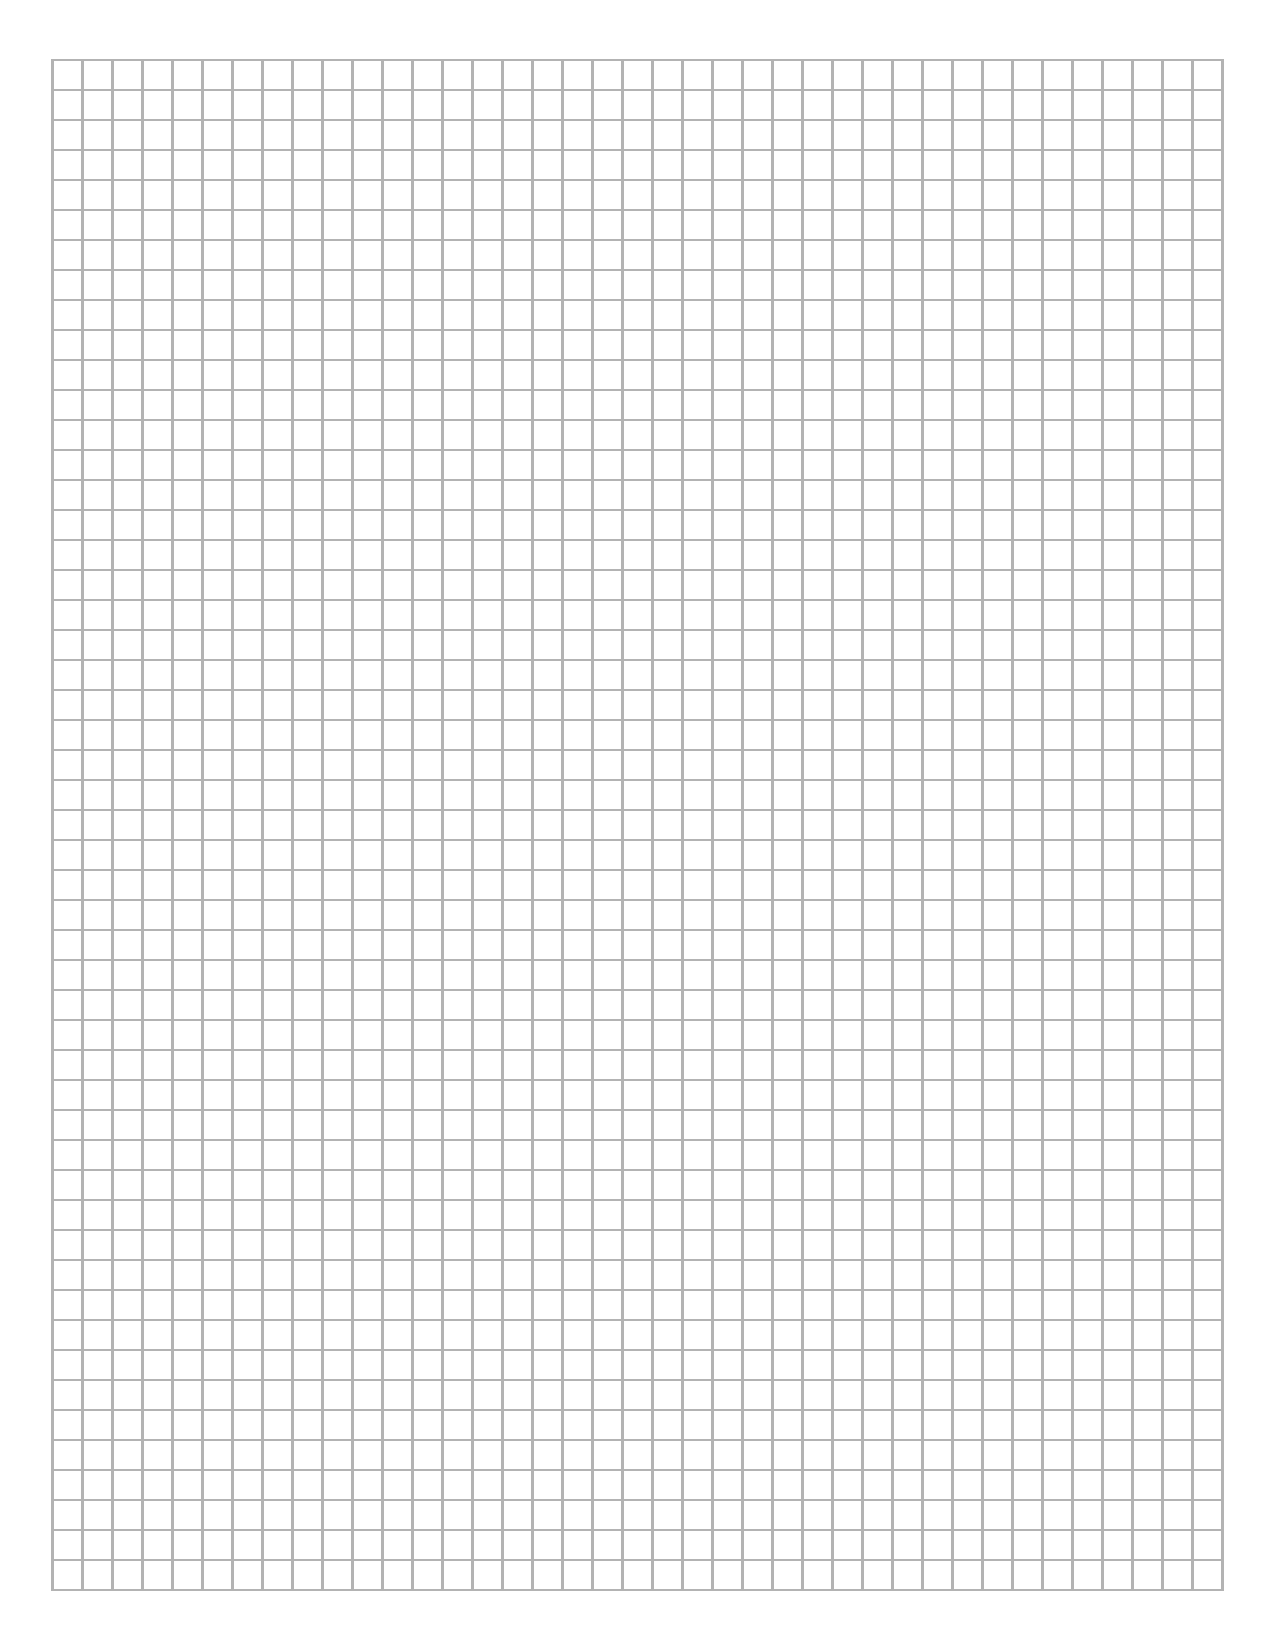
\includegraphics[width=\paperwidth,height=\paperheight,keepaspectratio]{/Users/jgates/desktop/latex/pics/plain.pdf}%
\vfill
}}}

%Diagram box command [v space][content]
\newcommand{\diagrambox}[2][40 mm]{
\framebox{\parbox{175 mm}{#2 \hfill \\ \vspace{#1}}}

\bigskip
}

% MakeList: [example number] [content]
\newcommand{\MakeList}[2]{
\begin{enumerate}[#1] \itemsep1pt \parskip0pt \parsep0pt  

#2
\end{enumerate}
}

\begin{document}



{\Large Problems tagged with standards:}Vectors
\bigskip 
% Number 1
% BFPM Tension FBD Vectors
% Hanging box, rope around 2 pulleys, theta = phi

% Watermark
\AddToShipoutPicture*{\BackgroundPic}

\addtocounter {ProbNum} {1}

\begin{floatingfigure}[r]{.2\textwidth}
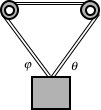
\includegraphics[scale=1]{/Users/jgates/desktop/latex/pics/hangingbox1.png}
\end{floatingfigure}
 
{\bf \Large{1.}} The box of mass ${6~kg}$ hangs at rest. 

\bigskip

\indent  a. Prove that ${\theta = \varphi}$.

\bigskip
b. Determine the tension in the rope, if ${\theta = 50^\circ}$.

\bigskip
\vspace{20mm}% Number 10
% Vectors
% Trig review - box leaning on wall
% MIT Physics for Teachers LON-CAPA

% Watermark
\AddToShipoutPicture*{\BackgroundPic}

\addtocounter {ProbNum} {1}

\begin{floatingfigure}[r]{.3\textwidth}
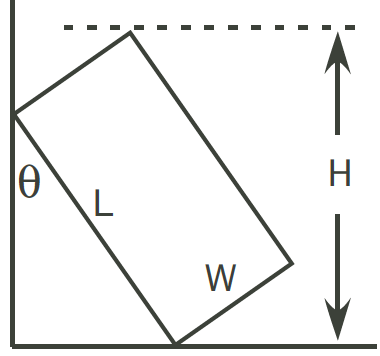
\includegraphics[scale=.4]{/Users/jgates/desktop/latex/pics/leaningbox.png}
\end{floatingfigure}
 
{\bf \Large{10.}} A rectangular box of length $L$ and width $W$ rests against a wall, making an angle $\theta$ with respect to the wall.  

\bigskip

\indent What is the height $H$ of the top edge of the box above the floor?

\bigskip
\vspace{20mm}% Number 60
% Vectors Relv
% Relative velocity - sailboat/wind
% MIT Physics for Teachers LON-CAPA

% Watermark
\AddToShipoutPicture*{\BackgroundPic}

\addtocounter {ProbNum} {1}

\begin{floatingfigure}[r]{.35\textwidth}
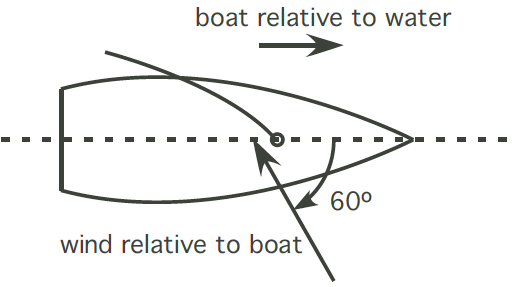
\includegraphics[scale=.4]{/Users/jgates/desktop/latex/pics/sailboat1.png}
\end{floatingfigure}
 
{\bf \Large{60.}} A sailboat is moving forward at a speed of 5 knots relative to the water. A gauge attached to its mast indicates a wind speed of 10 knots at an angle of 60 degrees, both relative to the boat. 
\bigskip

\indent What is the wind speed relative to the water?

\bigskip
\vspace{20mm}% Number 70
% Vectors UFPM
% Component of mg parallel to plane?
% MIT Physics for Teachers LON-CAPA

% Watermark
\AddToShipoutPicture*{\BackgroundPic}

\addtocounter {ProbNum} {1}

\begin{floatingfigure}[r]{.25\textwidth}
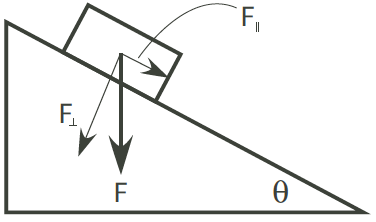
\includegraphics[scale=.4]{/Users/jgates/desktop/latex/pics/inclinedplane2.png}
\end{floatingfigure}
 
{\bf \Large{70.}} A gravitational force of magnitude F acts vertically downward on a block resting on a plane. The plane makes an angle of $\theta$ with the horizontal. 

\bigskip

\indent What is the magnitude of the component of the gravitational force acting parallel to the plane? 

\bigskip
\vspace{20mm}\end{document}